\documentclass{l4dc2026}
\usepackage{amsmath,amssymb,booktabs,graphicx,mathtools}
\usepackage{algorithm,algorithmic}
\jmlryear{2027}
\jmlrvolume{Under review}
\jmlrworkshop{L4DC 2027 --- Submission}
\title[Decision-Certified Compression]{Decision-Certified Compression for Safe Control\\with Unknown Linear Dynamics}
\author{\Name{Shivam Gupta} \Email{shivam1720406@gmail.com}\\\addr Independent Researcher}
\newcommand{\R}{\mathbb{R}}
\newcommand{\PN}{\mathcal P_N}
\newcommand{\PC}{\mathcal P_C}
\newcommand{\U}{\mathcal U}
\newcommand{\X}{\mathcal X}
\newcommand{\F}{\mathcal F}
\newcommand{\supp}{\operatorname{supp}}
\newcommand{\conv}{\operatorname{conv}}
\newcommand{\argmin}{\operatorname*{arg\,min}}
\raggedbottom
\emergencystretch=2em
\begin{document}
\maketitle
\begin{abstract}
Set-membership control accumulates a growing collection of data constraints, although a particular control decision may depend on only a small part of that collection. We study compression of the decision rather than reconstruction of the entire model set. For unknown full matrices $A$ and $B$, selected data define an outer model set and feasible model witnesses define an inner set. Their safety filters give a computable sandwich around the full-data intervention cost. A safe action is accepted when this sandwich closes to a prescribed tolerance; otherwise an archive returns support witnesses and sparse dual certificates. We prove that both sides can be compacted after acceptance: for box state constraints and row-separable models, at most $2n(n+m)$ scalar data inequalities and $m$ row-model witnesses suffice for the current certificate, independently of history length. We also establish an action-error bound, finite exact refinement for polyhedral models, and the screening condition needed after new data arrive. A construction separates decision-specific compression from uniform preservation of model support. Experiments evaluate four multivariable plants, two bounded-noise regimes, streaming updates, closed-loop control, and histories of up to 8,192 transitions. The method is a deterministic certificate architecture built from classical duality and support reduction, with explicit limitations on local memory, archive work, and numerical verification.
\end{abstract}
\begin{keywords}data-driven control, set-membership identification, robust safety filters, decision certificates, data compression\end{keywords}

\section{Introduction}
A controller that learns unknown dynamics from bounded-noise transitions can represent every model consistent with its history. This avoids committing to an inaccurate point estimate, but the representation grows with time. On an embedded controller, storing and optimizing over this history can become more expensive than computing the action itself. Discarding data preserves robust safety if it enlarges the model set; it may, however, make the controller unnecessarily conservative. Conversely, retaining only plausible models can produce an inexpensive optimistic controller without certifying safety. Neither representation alone answers the operational question: \emph{is the action available locally safe, and how much intervention could access to the entire history save?}

We answer this question with \emph{decision-certified compression} (DCC). An archive stores the history. A controller retains two complementary objects: selected data inequalities, which certify safety, and models feasible for the full history, which certify a lower bound on the best full-data intervention cost. Both bounds are evaluated at the current state and reference command. Their gap is an acceptance test, not a parameter-estimation error proxy. A query that fails the test triggers archive refinement; a query that passes needs no full-history optimization. Figure~\ref{fig:architecture} summarizes the architecture.

\begin{figure}[t]
\centering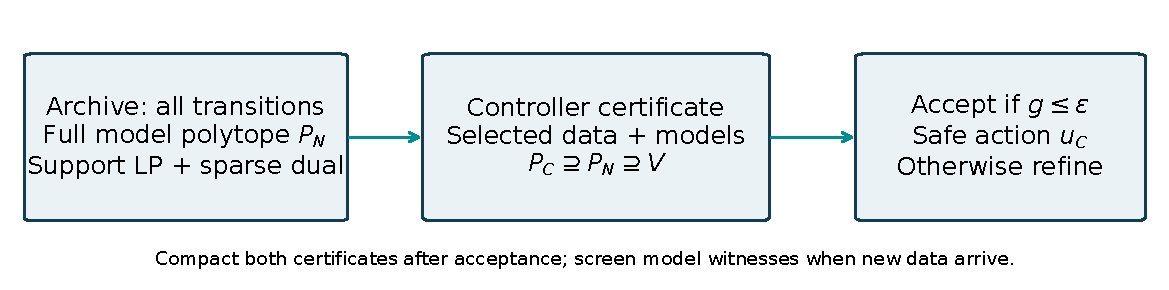
\includegraphics[width=\linewidth]{figures/architecture.pdf}
\caption{Two-sided local certificates. Enlarging the model set restricts safe actions; restricting the model set relaxes them. This reversal supplies an upper and a lower control-cost bound. The archive remains available when a new query needs more information.}\label{fig:architecture}
\end{figure}

The distinction from model compression is essential. A bounded-size summary need not preserve every future support query. We show that even a two-parameter model set can require arbitrarily many transitions for exact uniform preservation. Nevertheless, one accepted decision has a certificate whose size depends only on the state, input, and facet dimensions. The certificate can be reused, but its ability to certify a different decision must be checked again. This is a bound on \emph{retained controller information}, not on archive storage, refinement iterations, or computation independent of history length.

Our contributions are the coupled outer-data/inner-model acceptance rule for full-matrix robust control; simultaneous sparsification of its upper and lower certificates; a support-oracle refinement procedure with finite exact termination; and an append-only validity rule with a counterexample to stale reuse. We evaluate certificate validity, conservatism, communication proxies, timing, and physical closed-loop trajectories. We do not claim a new LP sparsity theorem, a new identification rate, or stability from a one-step intervention objective.

\section{Related Work and Positioning}
Set-membership identification describes unknown dynamics through all models consistent with bounded disturbances. \citet{li2024sets} analyze non-asymptotic uncertainty-set convergence. DCC requires containment of the true dynamics, but neither persistent excitation nor shrinking uncertainty for its per-decision guarantees. Such assumptions become relevant to how informative the archive is, rather than to whether the sandwich is valid.

The closest model-compression work is \citet{li2026coreset}. They select streaming transitions using geometric contraction of a polyhedral feasible set, with convergence and approximation guarantees for identification. DCC instead tests the current control objective using two different summaries of the same set. It may discard an identification-important constraint when that constraint is unnecessary for the current certificate. This does not preserve the feasible-set volume, Hausdorff error, or future decisions uniformly. The distinction is about the certified object, not the invention of dynamic-system coresets. Our fixed-budget heuristics are explicitly defined comparisons; they are not reproductions of the centroid-volume algorithm in that work.

Bounded-size optimization bases and exchange of active constraints are established ideas. Constraints consensus develops finite convergence and small-memory representations for abstract and convex optimization \citep{notarstefano2011,carlone2012}. Scenario optimization also uses support constraints, but yields probabilistic generalization guarantees under its sampling assumptions \citep{calafiore2006}. We use deterministic set containment: a retained data inequality is valid because it came from the archive, and a model witness is valid because it satisfies the archive. Sparse LP dual solutions, KKT conditions, and conic Carath\'eodory arguments are classical \citep{boyd2004}. The additional object here is a reusable pair of \emph{oppositely directed model summaries}, jointly compacted to retain a safe control-cost certificate and screened under subsequent data.

Safety filters minimally modify proposed commands to meet constraints \citep{wabersich2021}. Data-driven MPC addresses richer finite-horizon objectives and stability guarantees \citep{berberich2021}; our one-step filter assumes a known robustly invariant safe set. Data-driven certificate synthesis also uses compression for learned certificates and statistical guarantees \citep{rickard2026}. Our certificate is instead an optimization bound for a particular control query under a deterministic bounded-noise model. These distinctions constrain the scope of the novelty claim.

\section{Problem Formulation}
Consider
\begin{equation}\label{eq:dynamics}
 x_{t+1}=Ax_t+Bu_t+w_t=\Theta z_t+w_t,\qquad
 z_t=[x_t^\top,u_t^\top]^\top,\quad |w_{t,i}|\leq\eta_i,
\end{equation}
where $x_t\in\R^n$, $u_t\in\R^m$, $d=n+m$, and every entry of $\Theta=[A\ B]$ may be unknown. States are measured exactly. A known compact polyhedral prior $\mathcal P_0$ contains the true $\Theta$. From $N$ transitions $(z_t,y_t=x_{t+1})$, define the nonempty compact set
\begin{equation}\label{eq:set}
 \PN=\{\Theta\in\mathcal P_0:|y_{t,i}-\theta_i^\top z_t|\leq\eta_i\ \text{for all }t,i\}.
\end{equation}
For the main construction the prior is row-separable, so $\PN=\prod_i P_{N,i}$, with
\begin{equation}\label{eq:row}
 P_{N,i}=\{\theta\in\R^d:C_i\theta\leq b_i\}.
\end{equation}
Prior constraints are always retained. A \emph{data inequality} is one signed scalar side of a transition slab; a raw transition generates $2n$ such inequalities. Counts of these objects are not interchangeable.

Let $\X=[-1,1]^n$ and $\U=[-\bar u,\bar u]^m$. For a model set $P$, define
\begin{equation}\label{eq:feasible}
 \F(P,x)=\{u\in\U:\Theta[x;u]+w\in\X\ \ \forall\Theta\in P,\ |w_i|\leq\eta_i\}.
\end{equation}
The full-data filter projects a reference $v\in\R^m$:
\begin{equation}\label{eq:filter}
 u_N=\argmin_{u\in\F(\PN,x)}f_v(u),\qquad
 f_v(u)=\tfrac12\|u-v\|_2^2,\quad J_N=f_v(u_N).
\end{equation}
The objective measures command intervention, not accumulated tracking error or energy consumption. Strict convexity makes $u_N$ unique.

\paragraph{Feasibility assumption.}
A supplied backup $\kappa(x)\in\U$ satisfies $\kappa(x)\in\F(\mathcal P_0,x)$ for every $x\in\X$. Hence every outer model set contained in $\mathcal P_0$ has a feasible filter. Starting in $\X$, robust feasibility at every step implies forward invariance of $\X$ by induction. This assumption is substantive; DCC does not learn the invariant set or its backup.

\section{Two-Sided Decision Certificates}
Let $C$ select data inequalities and let $P_{C,i}$ retain those inequalities together with the prior. Then $P_{N,i}\subseteq P_{C,i}$. Let $V_i\subseteq P_{N,i}$ be finitely many row-model witnesses, possibly empty. Define
\begin{align}
 \F_C(x)&=\left\{u\in\U:\max_{\theta\in P_{C,i}}s\theta^\top[x;u]\leq1-\eta_i,\ \forall i,s\in\{-1,1\}\right\},\label{eq:outer}\\
 \F_V(x)&=\{u\in\U:s\theta^\top[x;u]\leq1-\eta_i,\ \forall i,s,\theta\in V_i\}.\label{eq:inner}
\end{align}
Empty witness sets impose no model constraints. Row witnesses suffice because the uncertainty is separable; a coupled prior instead requires whole-matrix witnesses. Let $u_C$ minimize $f_v$ over $\F_C$, with value $J_C$. Let $J_V$ be the corresponding minimum over $\F_V$.

\begin{theorem}[Decision sandwich]\label{thm:sandwich}
Under the preceding assumptions,
\begin{equation}\label{eq:sandwich}
 \F_C(x)\subseteq\F(\PN,x)\subseteq\F_V(x),\qquad
 \ell\leq J_V\leq J_N\leq J_C,
\end{equation}
for any valid dual lower bound $\ell$ for the optimistic filter. Consequently, $u_C$ is robustly safe and $g=J_C-\ell$ certifies
\begin{equation}\label{eq:action}
 0\leq f_v(u_C)-J_N\leq g,\qquad \|u_C-u_N\|_2\leq\sqrt{2g}.
\end{equation}
\end{theorem}
\begin{proof}
Universal constraints reverse model-set containment, giving the feasible-set inclusions and objective bounds. Projection optimality gives $(u_N-v)^\top(u_C-u_N)\geq0$. Expanding the quadratic then gives $f_v(u_C)-f_v(u_N)\geq\frac12\|u_C-u_N\|^2$, which proves the action bound.
\end{proof}

The lower certificate need not solve the optimistic QP exactly. Write its constraints, including input bounds, as $Hu\leq h$. Every $\lambda\geq0$ yields the weak-duality lower bound
\begin{equation}\label{eq:dualqp}
 \ell(\lambda)=\lambda^\top(Hv-h)-\tfrac12\|H^\top\lambda\|_2^2.
\end{equation}
A feasible outer action and any such lower bound suffice for acceptance when $g\leq\epsilon$. Exact minimizers are needed only for the optimum-preservation and sparse KKT statements below, not for validity of a conservative sandwich.

\subsection{Compacting both sides}
For each outer safety face $(i,s)$, a support LP at $z_C=[x;u_C]$ has dual
\begin{equation}\label{eq:dualLP}
 \max_{\theta\in P_{C,i}}(s z_C)^\top\theta
 =\min_{\alpha\geq0}\{b_{C,i}^\top\alpha:C_{C,i}^\top\alpha=s z_C\}.
\end{equation}
A basic optimal dual can use at most $d$ positive multipliers. Let $C'$ retain their data inequalities over all $2n$ faces, together with the prior. Although $P_{C'}$ is larger, these duals still certify feasibility of $u_C$.

\begin{theorem}[Two-sided compaction]\label{thm:compact}
In exact arithmetic, an accepted certificate with exact outer and optimistic minimizers has a compact representation with at most $2nd$ selected scalar data inequalities and at most $m$ row-model witnesses. It preserves $J_C$, $J_V$, and the accepted action. Prior and input constraints are retained separately. The number of distinct retained raw transitions is also at most $2nd$, but can be smaller. For a full, possibly coupled model polytope of dimension $D$ and a polyhedral safe set with $q$ facets, the analogous bounds are $qD$ scalar data inequalities and $m$ whole-model witnesses.
\end{theorem}
\begin{proof}
An optimal basic support dual uses at most the dimension of its variable space. Taking the union over faces gives $2nd$ (or $qD$). Since fewer data enlarge the model set, they shrink the feasible action set: the new optimal cost cannot fall below $J_C$. The retained duals certify that the old action is still feasible, so the cost cannot rise either.

For the optimistic QP, stationarity represents $v-u_V$ as a conic combination of active model-constraint normals and active input-bound normals in $\R^m$. Conic Carath\'eodory gives a representation using at most $m$ normals in total. Keep the associated model witnesses and all input bounds. Primal feasibility, complementary slackness, and stationarity still hold, so $u_V$ remains optimal. There are at most $m$ distinct retained witnesses. For a coupled polytope the same argument uses full-model facet normals.
\end{proof}

This proof combines standard LP and QP support reductions \citep{boyd2004}; the useful control object is their joint preservation of both sides of~\eqref{eq:sandwich}. A retained witness carries a row vector of length $d$, whereas a retained data inequality carries a normal and offset. The controller's stored scalar payload is therefore $O(nd^2+md)$ plus the prior, not $O(nd)$ bytes. The theorem bounds the \emph{post-acceptance} cache; temporary refinement memory can grow.

\subsection{Archive refinement and reuse}
The archive solves $2n$ full-history support LPs at the current optimistic action. If a witness violates a safety face, it is added to $V_i$ and its sparse support-dual data inequalities are added to $C$. If no face is violated but the sandwich remains open, all support bases are added. These make the optimistic action feasible for the outer filter, closing the exact gap. Algorithm~\ref{alg:dcc} states the procedure.

\begin{algorithm}[t]
\caption{Decision-certified compression (exact-arithmetic specification)}\label{alg:dcc}
\begin{algorithmic}[1]
\REQUIRE Prior-containing history set $P_N$, selected data $C$, valid witnesses $V$, query $(x,v)$, tolerance $\epsilon\geq0$
\LOOP
\STATE Solve outer filter for $(u_C,J_C)$ and optimistic filter for $(u_V,J_V)$.
\IF{$J_C-J_V\leq\epsilon$}
\STATE Compact data by support duals at $u_C$ and witnesses by KKT support at $u_V$.
\RETURN $u_C$ and certificate $(J_C,J_V)$.
\ENDIF
\STATE Archive maximizes each safety-face support at $[x;u_V]$.
\STATE Add violating maximizing models and their support-dual data bases.
\STATE If none violates, add all returned support-dual bases.
\ENDLOOP
\end{algorithmic}
\end{algorithm}

\begin{proposition}[Finite exact refinement]\label{prop:finite}
If support oracles return vertices of a fixed compact polytope and no compaction occurs within a query, Algorithm~\ref{alg:dcc} terminates for $\epsilon=0$ after finitely many refinements. The same conclusion holds for every $\epsilon>0$.
\end{proposition}
\begin{proof}
A violating vertex cannot already be a retained witness, since $u_V$ satisfies every retained witness constraint. Each violating round therefore adds a new vertex from a finite collection. If a round has no violation, support duals make $u_V$ feasible for the enlarged-uncertainty outer filter. Its objective is the optimistic lower bound, so the sandwich closes in the next iteration.
\end{proof}
No polynomial iteration bound follows: a polytope may have many vertices. Exact duplicate handling, fixed-history validity, and vertex-returning oracles are part of this statement. The implementation uses tolerances, conservative safety margins, and finite iteration caps, and records a failure rather than asserting convergence after a cap.

\section{What the Certificate Does and Does Not Preserve}
\subsection{New data invalidate some lower witnesses}
For append-only histories, $P_{N+1}\subseteq P_N$. Previously selected data remain an outer representation, hence their actions remain safe. Previously feasible model witnesses may leave the new model set. Retaining such a witness can make the optimistic problem \emph{more restrictive} than the new full-data problem, invalidating its claimed lower bound. Screen every cached row witness against every new slab before reusing it; discard any violator. Full-history support calls subsequently produce valid replacements. With unchanged prior and disturbance bounds, this restores all inclusions in Theorem~\ref{thm:sandwich}.

The explicit counterexample in Appendix~\ref{app:additional} shows that an apparently zero gap can conceal an actual cost gap of $0.06$.

\subsection{Decision compression is weaker than model preservation}
\begin{proposition}[Unbounded exact uniform summaries]\label{prop:polygon}
Even for $n=m=1$, there are bounded-noise transition sets for which retaining all model support directions exactly requires arbitrarily many raw transitions, while Theorem~\ref{thm:compact} bounds a single decision certificate.
\end{proposition}
A regular-polygon construction proves the claim (Appendix~\ref{app:additional}).

This construction is about information preservation, not about safety-filter feasibility with $\eta=1$. It precludes interpreting the decision bound as an exact, fixed-size identification coreset.

\section{Experimental Design}\label{sec:experiments}
The public implementation and retained results are at \url{https://github.com/shi1720/decision-certified-control}. The evaluation plan precedes the main runs and records the pilot amendment used to activate safety constraints. All methods, queries, and failures are retained. Appendix~\ref{app:plants} supplies matrices and generators; Appendix~\ref{app:numerics} supplies tolerances and independent checks.

\paragraph{Systems and data.}
The primary study uses a four-state thermal network with two inputs, a normalized mechanical-inspired $(4,2)$ plant, a nonnormal $(6,2)$ plant with open-loop instability and a known linear backup, and a dense stable $(8,3)$ plant. Every entry of both $A$ and $B$ is uncertain. The box-prior radius is $0.12/(n+m)$ per entry; true entries are sampled independently within $70\%$ of this radius. Process-noise bounds are $\eta_i=0.015$, state bounds are one, and input bounds are $0.8$. There are 12 independent plant/noise seeds for each of two noise regimes: uniform in the box, or independent signs at its boundary. Each of the 96 histories contains 1,024 actual sequential transitions, generated with prior-safe inputs. Boundary noise is included because geometric selection can depend strongly on which constraints are informative.

\paragraph{Common-query comparisons.}
For each history, all methods answer the same 96 state and reference queries. One quarter use random interior states and reference commands; three quarters align a near-boundary state and aggressive reference with a randomly selected nominal dynamics row. These are declared stress queries, not claimed stationary deployment samples. We compare the full-data filter, DCC with $\epsilon=10^{-5}$ and $10^{-3}$, and random, greedy log-determinant, rolling-window, and prior-only outer-data filters. Fixed-budget methods retain $k=\min(N,2n(n+m))$ \emph{whole transitions}, hence up to $2nk$ scalar data inequalities. This gives them more scalar constraints than DCC; actual counts are reported. Random selection is without replacement. Log-determinant selection greedily maximizes regressor leverage from a $10^{-6}I$ ridge, and does not use response offsets. None of these baselines has a DCC-style full-data cost certificate.

\paragraph{Secondary studies.}
Closed-loop simulations use three independent seeds per plant and noise regime, 96 steps per method, held reference patterns, and shared disturbance tapes. Policy trajectories differ, so their cumulative intervention is not interpreted as a paired same-query regret. Streaming uses three seeds per plant, histories of 64, 128, 256, 512, and 1,024 transitions, and 12 queries at every update; a standalone controller reconstructs each action from the exported certificate alone. Ablations disable post-query compaction or reset the cache before every query. A scaling study varies $n\in\{2,4,8,12\}$ and $N\in\{128,512,2048,8192\}$ with two inputs, three seeds, and 16 queries per condition. Timing includes optimization but excludes one-time fixed-subset selection; all solvers run locally, without simulated network delay. We distinguish controller time, archive time, and total time.

\paragraph{Statistics and audit.}
The primary study contains 9,216 distinct queries and 64,512 method-query evaluations. Mean excess intervention is paired against the independently solved full-data filter at each query. Confidence intervals resample the 12 whole seeds per plant, grouping both disturbance regimes and all queries within each seed; they describe simulation variation for this specified benchmark distribution. We check dynamics residuals, prior/noise containment, input and successor bounds, sandwich inequalities, action bounds, and retained support counts. The experiment code uses floating-point primal/dual residual checks, not interval arithmetic. Consequently the mathematical guarantees are exact-arithmetic theorems, and the computational evidence is verification to declared tolerances.

\section{Results}\label{sec:results}
All primary solves and all 168 closed-loop episodes completed without recorded solver failures. The maximum true-model bounded-noise successor and selected-set robust successor were both $0.9999999701$ or lower; all inputs satisfied their bounds to numerical tolerance. The 18,432 DCC evaluations satisfied the gap thresholds, sandwich inequalities, action bounds, and post-compaction support counts. Maximum lower-bound excess over the full-data objective was $4.1\times10^{-14}$, and maximum excess over the action-error bound was $1.7\times10^{-13}$. These residuals support numerical consistency, not exact floating-point certification.

\paragraph{Conservatism and retained information.}
At $\epsilon=10^{-3}$, mean excess cost was $6.94\times10^{-6}$ over all plants; the maximum was $9.73\times10^{-4}$. At $10^{-5}$, the mean was $8.99\times10^{-9}$ and maximum below $7\times10^{-6}$. Table~\ref{tab:main} and Figure~\ref{fig:performance} separate plants. DCC retained a mean of 44.0 scalar data inequalities at $10^{-3}$, versus 11,264 for full histories averaged over plants, plus the excluded fixed prior. The largest observed count was 152, below each plant's $2n(n+m)$ bound. DCC retained at most two witnesses for the two-input plants and one for the three-input dense plant.

Fixed-budget data subsets had larger average excess costs under uniform noise: $0.0255$ for random, $0.0189$ for log-determinant, and $0.0275$ for rolling-window selection. Under boundary noise all three matched the full-data filter up to numerical error. This negative control matters: the method is not uniformly more accurate than subset heuristics. Here, informative boundary samples made even small subsets effectively exact. DCC supplies a per-query certificate in either regime rather than assuming that informativeness.

\paragraph{Archive access and timing.}
At $10^{-3}$, queries accepted without archive calls ranged from $29.6\%$ for the nonnormal plant to $91.2\%$ for the dense plant. Mean total times were 22.5, 12.4, 55.6, and 15.1\,ms, versus 48.7, 35.4, 111.9, and 100.1\,ms for full data. DCC was generally slower than fixed-budget heuristics, except in the dense case. Its tradeoff is certified conservatism and lower retained information, not universal speed. These local wall times include archive work, omit real network latency, and are affected by concurrent computation. Appendix tables expose the local/archive split.

\paragraph{Scaling, reuse, and streaming.}
Scaling retained at most 15, 47, 139, and 256 inequalities for $n=2,4,8,12$, below bounds 16, 48, 160, and 336. At $n=12$, increasing the archive from 128 to 8,192 transitions increased mean full-data time from 32.7\,ms to 2.83\,s and DCC total time from 25.8\,ms to 0.793\,s. Archive computation still grows with history length (Figure~\ref{fig:cert}).

Resetting the cache before each ablation query used 8.33 archive LPs per query on average; reuse with compaction used 6.45. Disabling compaction reduced this to 2.47 but increased retained data from 29.4 to 44.5 inequalities on average over short 32-query sequences. Aggressive compaction can therefore sacrifice future reuse. An input-box-only lower bound, omitting model witnesses, gave a mean certificate gap of $0.474$, although the two-sided gap was below $10^{-4}$. Optimistic witness-only actions violated a full-model face in eight ablation queries (maximum $2.78\times10^{-5}$), demonstrating why a lower certificate alone is insufficient for safety.

Across 720 streaming queries, screening invalidated 41 cached row witnesses. Actions reconstructed from exported payloads alone agreed with archive-backed actions within $3\times10^{-14}$; all reconstructed gaps met $10^{-4}$ to tolerance. At 1,024 transitions, the median JSON payload/raw-float64-data ratio was $0.104$; short histories can have ratios above one (Figure~\ref{fig:ablation}). The stale-witness example produced a near-zero claimed gap but an actual gap of $0.06$ before screening.

\paragraph{Closed loop.}
All 16,128 physical control steps remained in the safe box, with maximum coordinate magnitude below $0.9999999701$. Mean cumulative intervention per 96-step episode was 139.713411 for full data and DCC at $10^{-5}$, and 139.713333 for DCC at $10^{-3}$. The latter can be smaller because policy trajectories differ; it is not a violation of common-query optimality. Prior-only control had mean intervention 139.760339. These small differences indicate that primary stress-query improvements do not translate into a large closed-loop intervention improvement in this deployment experiment.


\begin{figure}[t]
\centering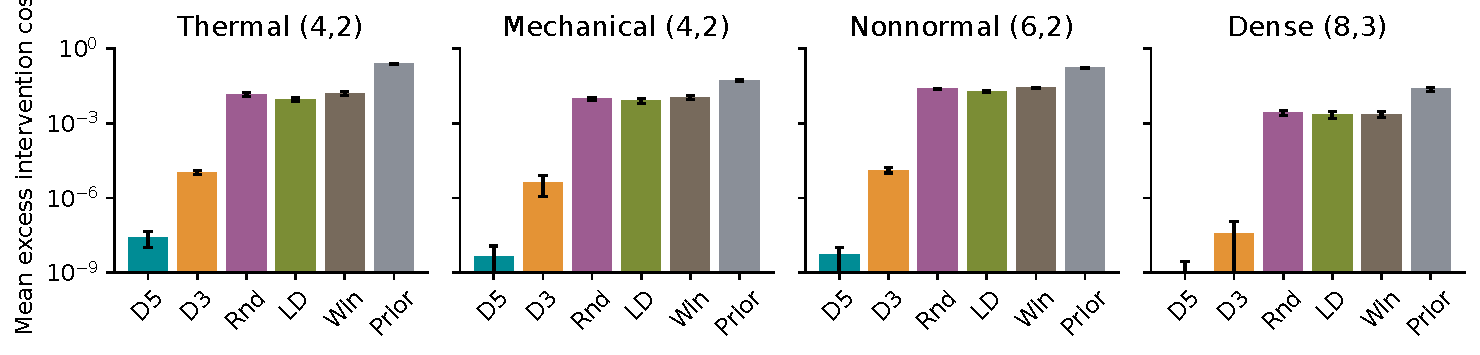
\includegraphics[width=\linewidth]{figures/performance.pdf}
\caption{Excess command-intervention cost against the same-query full-data filter. D5/D3 denote DCC tolerances $10^{-5}/10^{-3}$; Rnd, LD, and Win denote random, log-determinant, and rolling-window selection. Bars show means; intervals bootstrap independent seeds. A logarithmic axis exposes small certificate-controlled errors. These are deliberately constraint-activating simulation queries.}\label{fig:performance}
\end{figure}

\begin{table}[t]\centering\small
\caption{Primary study at DCC tolerance $10^{-3}$. Mean excess cost, mean selected scalar data inequalities, and mean total time including archive work. LD is the fixed-budget log-determinant baseline; its data count is larger. Full plant/method intervals appear in Appendix Table~\ref{tab:main}.}\label{tab:compact}
\begin{tabular}{lrrrrr}\toprule
Plant & DCC gap & LD gap & DCC data & LD data & DCC/full ms\\\midrule
Thermal & $1.05\!\times\!10^{-5}$ & 0.00897 &31.7&384&22.5/48.7\\
Mechanical & $4.16\!\times\!10^{-6}$ &0.00784&13.4&384&12.4/35.4\\
Nonnormal & $1.31\!\times\!10^{-5}$ &0.01887&59.3&1152&55.6/111.9\\
Dense & $3.81\!\times\!10^{-8}$ &0.00219&71.7&2816&15.1/100.1\\\bottomrule
\end{tabular}\end{table}

\begin{figure}[t]
\centering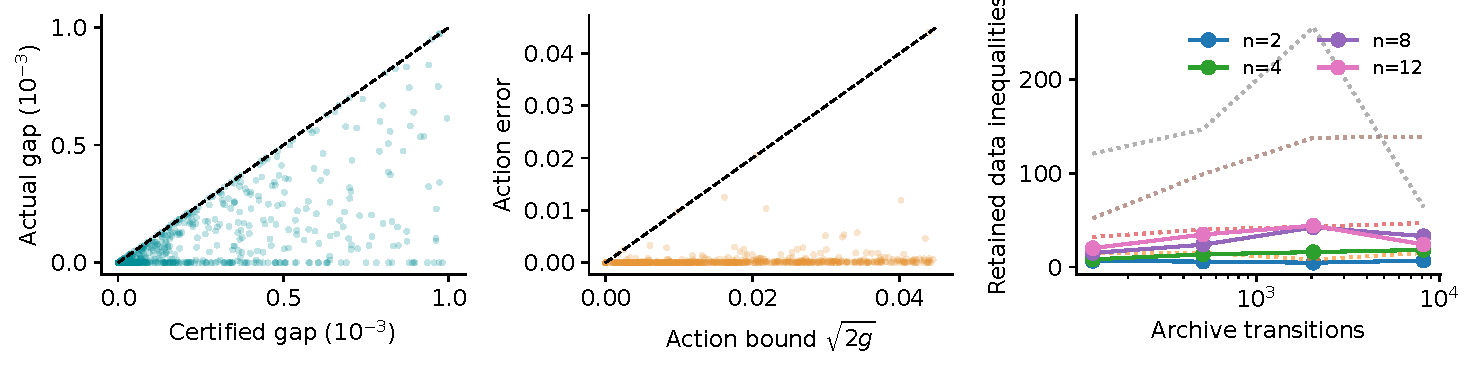
\includegraphics[width=\linewidth]{figures/certificates_scaling.pdf}
\caption{Left: certified versus actual cost gaps for DCC at $10^{-3}$. Center: action error versus its strong-convexity bound. Dashed lines are equality. Right: post-acceptance selected data inequalities in the scaling study (solid means, dotted maxima). A history-independent bound does not imply that observed support size is constant or that archive computation is independent of history.}\label{fig:cert}
\end{figure}



\section{Discussion and Limitations}
DCC targets controllers whose full history is in remote or slower storage. A certificate service could support edge safety filters in building or industrial control when a conservative backup and state/input limits are available. This is an application hypothesis: we do not measure hardware latency, commercial demand, savings, or patentability. Short histories can require larger certificates than raw data, and novel queries can repeatedly contact the archive.

Exact states, known disturbance bounds, a containing prior, and a supplied invariant set are required. Underestimated noise or changing dynamics can invalidate safety. Changing the prior or noise bound requires rebuilding certificates; append-only screening alone is insufficient. Measurement uncertainty needs an errors-in-variables outer model. Multi-step objectives, output feedback, nonlinear models, and interrupted refinement remain open. A backup preserves safety while waiting, but does not inherit the requested cost gap.

The simulated plants have modest dimensions and hand-specified priors. They establish behavior in controlled settings rather than industrial readiness. We do not implement the geometric centroid-volume coreset algorithm and therefore cannot rank DCC against its runtime or identification quality. Our comparison evaluates a decision guarantee against the full-data optimum and transparent subset baselines. Measured-state application studies with verified noise bounds and hardware scheduling are needed to establish deployment value.

\section{Conclusion}
Selected data and feasible model witnesses jointly certify the safety and intervention cost of a decision under unknown full dynamics. Dual and KKT supports bound the retained certificate size; archive refinement and witness screening handle new queries and data. The experiments demonstrate this tradeoff while exposing its archive burden and deployment assumptions.

\clearpage
\bibliography{references}
\appendix
\section{Benchmark Matrices and Feasibility}\label{app:plants}
Write $\bar\Theta=[\bar A\ \bar B]$, and let $r=0.12/(n+m)$. All true entries are $\bar\Theta_{ij}+r\xi_{ij}$, $\xi_{ij}\sim\operatorname{Uniform}[-0.7,0.7]$. The prior is $|\Theta_{ij}-\bar\Theta_{ij}|\leq r$. A seed fixes a plant realization and its disturbance tape; the same integer seed across two disturbance regimes does not create a separate parameter draw, so regime-specific comparisons should not be interpreted as independent realizations of the dynamics. Bootstrap intervals group both regimes and all queries by the 12 independent seeds per plant. They therefore preserve this shared-parameter dependence.

For the thermal plant,
\[
 L=\begin{bmatrix}2&-1&0&-1\\-1&2&-1&0\\0&-1&2&-1\\-1&0&-1&2\end{bmatrix},\quad
 \bar A=e^{-0.2I-0.12L},\quad
 \bar B=0.4\begin{bmatrix}1&0\\0.7&0.2\\0&1\\0.2&0.7\end{bmatrix}.
\]
For the mechanical-inspired plant,
\[
 G=\begin{bmatrix}0_{2\times2}&I_2\\-M&-0.9I_2\end{bmatrix},\quad
 M=\begin{bmatrix}2&-0.4\\-0.4&1.5\end{bmatrix},\quad
 \bar A=0.72\,e^{0.3G}/\|e^{0.3G}\|_\infty,\quad
 \bar B=\begin{bmatrix}0.12I_2\\0.55I_2\end{bmatrix}.
\]
Normalization gives a convenient prior-safe benchmark; it is not the exact discretization of a specified physical mechanism after normalization. For the nonnormal plant, $F=0.7I_6+0.14\operatorname{diag}(1,1,1,1,1;1)$ (the second term is the superdiagonal),
\[
 \bar B=1.5\begin{bmatrix}0.5&0\\0.3&0.1\\0.1&0.35\\0.35&-0.1\\0.1&0.45\\-0.1&0.3\end{bmatrix},\quad
 K=\begin{bmatrix}-0.6&0&0&0&0&0\\0&0&0&0&-0.6&0\end{bmatrix},\quad \bar A=F-\bar BK.
\]
The dense plant uses NumPy's default generator with seed 887, drawing a standard-normal $8\times8$ matrix followed by an $8\times3$ matrix. Normalize the first to induced infinity norm $0.65$ and the second to maximum row absolute sum $0.65$. Use $K=0$ for the other three plants.

For $x\in\X$, the backup $Kx$ satisfies $\|Kx\|_\infty\leq\|K\|_\infty\leq0.8$. For each row,
\begin{equation}
 |((A+BK)x)_i|+\eta_i\leq
 \| (\bar A+\bar BK)_{i,:}\|_1+r\left(n+\sum_{j,k}|K_{jk}|\right)+\eta_i<1.
\end{equation}
The code independently checks these inequalities. During data generation, sample a bounded exploratory input and repeatedly average it with $Kx$ until the prior support bound plus noise is below one. This supplies real sequential transitions, not independently sampled regression rows. The benchmark is identification of full matrices inside a prior that already supplies safe exploration; it does not solve safe exploration without prior knowledge.

The scaling family uses $\bar A=0.65I_n$, a Gaussian two-input $\bar B$ normalized to maximum row absolute sum $0.8$, the same radius/noise model, and a zero backup. Its generator and seeds are retained separately from the four-plant primary experiment.

\section{Numerical Implementation and Verification}\label{app:numerics}
The reference implementation uses Python, NumPy, and SciPy \citep{virtanen2020}. Support LPs use HiGHS via \texttt{scipy.optimize.linprog}; the underlying simplex methods are described by \citet{huang2018}. Variables are explicitly free, avoiding the library's default nonnegativity bounds. The robust projection is a cutting-plane exchange of support constraints around a small Euclidean-projection QP, solved by SLSQP. QP multipliers are obtained from a nonnegative stationarity LP over active constraints, with NNLS fallback. The reported optimistic lower bound always uses~\eqref{eq:dualqp}; a solver success flag alone is not treated as a certificate.

For each support LP, the code checks primal violation, dual stationarity residual, and absolute primal-dual gap against $10^{-7}$; the LP feasibility tolerances are $10^{-9}$. QP primal violation must be at most $10^{-7}$, stationarity residual at most $2\times10^{-6}$, and lower bound no larger than primal value plus $10^{-7}$. Active constraints use slack below $2\times10^{-7}$, and dual supports use positive-weight cutoffs of $10^{-10}$ (LP) and $10^{-9}$ (QP). These cutoffs are numerical approximations to exact sparsity and are checked empirically after compaction. Every robust safety face includes a $3\times10^{-8}$ inward margin. The exchange loop stops when the worst face residual is at most $2\times10^{-9}$, with caps of 120 outer exchanges and 100 certificate refinements. An accepted DCC gap must be at most $\epsilon+10^{-9}$.

The theorem compares filters with identical safety sets. In code the full, outer, and optimistic filters all use the same inward margin, so the reported cost comparison is for that margin-tightened problem. None of these floating-point checks is an interval certificate. A deployment demanding machine-verifiable safety should outward-round support upper bounds or use exact/rational certificates and account for state and actuator uncertainty.

Independent checks include 80 support problems whose two-dimensional vertices are enumerated from every pair of inequalities; 100 one-input QPs compared with analytic feasible intervals; 45 matrix-valued queries checking sandwich/action bounds and zero archive calls on immediate repeated queries after compaction; prior-safe backup checks for all plants; witness screening; every-facet irredundancy for regular polygons with 4, 8, 16, and 32 transition slabs; and append-ID remapping plus portable-controller reconstruction on distinct seeds. The complete result audit recomputes objectives from retained query/action arrays and verifies sequential training dynamics and true-model containment. The streaming benchmark reconstructs 720 actions from payloads containing only selected inequalities, witnesses, dimensions, input bounds, and noise bounds. It has no access to the full archive when solving those local filters.

\section{Additional Results and Reproduction}\label{app:additional}
Primary seeds are 2000--2011. Closed-loop, streaming, ablation, and scaling seeds are disjoint ranges 3000--3002, 4000--4002, 5000--5001, and 6000--6002. Geometry tests use separate seeds. A design pilot used eight queries per plant, motivated the declared boundary-query mixture, and is excluded from final statistics. No runs were discarded for unfavorable results. An initial performance pilot was stopped to remove redundant full-history audits from comparator timing; the entire primary study was then rerun under the frozen scientific specification.

\begin{table}[ht]\centering
\caption{DCC at $10^{-3}$: data retention, archive access, and mean time (ms). Prior and input constraints are always retained.}\label{tab:timing}
\setlength{\tabcolsep}{5pt}
\begin{tabular}{lrrrrrr}\toprule
Plant & Data mean & Data max & Local hit (\%) & Local ms & Archive ms & Full ms\\\midrule
Thermal &31.7&47&43.4&7.62&14.90&48.69\\
Mechanical &13.4&47&69.4&4.71&7.74&35.39\\
Nonnormal &59.3&87&29.6&16.50&39.11&111.95\\
Dense &71.7&152&91.2&7.13&7.99&100.08\\\bottomrule\end{tabular}\end{table}

\begin{table}[ht]\centering
\caption{Scaling endpoints. Mean retained scalar data inequalities and mean total query time (ms). Three seeds and 16 queries per seed; $m=2$. Intermediate lengths are retained in the repository.}\label{tab:scaling}
\begin{tabular}{rrrrr}\toprule
$n$ & $N$ & Data mean & Full ms & DCC ms\\\midrule
2&128&6.38&3.51&4.21\\2&8192&6.81&137.85&37.15\\
4&128&8.15&8.08&9.56\\4&8192&18.23&439.01&146.88\\
8&128&14.98&20.05&21.68\\8&8192&32.88&1121.67&340.70\\
12&128&20.08&32.75&25.78\\12&8192&23.94&2825.01&793.21\\\bottomrule\end{tabular}\end{table}

\paragraph{Noise regimes.}
Uniform-noise mean excess costs were $1.73\times10^{-8}$ and $1.34\times10^{-5}$ for DCC at $10^{-5}$ and $10^{-3}$. Boundary-noise means were $7.01\times10^{-10}$ and $4.62\times10^{-7}$. Fixed-budget methods had boundary-noise excess costs of order $10^{-16}$, while prior-only control remained conservative in both regimes (means $0.118$ and $0.126$). Noise regimes should therefore be reported separately.

\paragraph{Independent trajectory audit.}
The trajectory archive stores every state, input, reference, disturbance, and realized dynamics matrix for every closed-loop policy. Rechecking $x_{t+1}=\Theta[x_t;u_t]+w_t$ independently of the simulator verifies sequential consistency and state/input bounds. The primary training archive contains 98,304 transitions, excluding secondary training histories and rollouts. The 64,512 primary evaluations share 9,216 state/reference instances and must not be treated as independent statistical replicates.

\paragraph{Noise-envelope stress audit.}
Holding the 9,216 DCC ($10^{-3}$) query actions fixed, replace the deployment disturbance box by twice or five times the assumed bound. The true-model worst-case successor then exceeds the safe box in 4,666 or 4,832 queries, respectively, versus zero at the assumed bound. This is an adversarial envelope check, not a sampled disturbance violation rate or a retrained-controller comparison. It illustrates the need for a valid disturbance bound rather than claiming robustness to assumption violations.

\begin{table}[ht]
\centering\small
\caption{Common-query performance. Mean and 95\% seed-cluster bootstrap interval for excess cost, mean retained \emph{scalar data inequalities} (prior excluded), and mean total milliseconds per query including archive refinement. Fixed-budget methods retain whole transitions.}\label{tab:main}
\begin{tabular}{llrrrr}\toprule
Plant $(n,m)$ & Method & Mean gap & 95\% interval & Data & ms\\\midrule
Thermal (4,2) & DCC ($10^{-5}$) & 2.53e-08 & [9.8e-09,4.4e-08] & 31.8 & 25.9 \\
 & DCC ($10^{-3}$) & 1.05e-05 & [8.6e-06,1.2e-05] & 31.7 & 22.5 \\
 & Random & 1.42e-02 & [1.2e-02,1.7e-02] & 384.0 & 6.1 \\
 & Log-det & 8.97e-03 & [7.7e-03,1.0e-02] & 384.0 & 6.1 \\
 & Window & 1.57e-02 & [1.2e-02,1.9e-02] & 384.0 & 6.0 \\
 & Prior & 2.43e-01 & [2.3e-01,2.6e-01] & 0.0 & 4.1 \\
\midrule
Mechanical (4,2) & DCC ($10^{-5}$) & 4.57e-09 & [-4.3e-18,1.2e-08] & 14.8 & 13.2 \\
 & DCC ($10^{-3}$) & 4.16e-06 & [1.1e-06,8.1e-06] & 13.4 & 12.4 \\
 & Random & 9.80e-03 & [8.6e-03,1.1e-02] & 384.0 & 4.4 \\
 & Log-det & 7.84e-03 & [6.1e-03,9.7e-03] & 384.0 & 4.5 \\
 & Window & 1.10e-02 & [9.2e-03,1.3e-02] & 384.0 & 4.3 \\
 & Prior & 4.98e-02 & [4.6e-02,5.5e-02] & 0.0 & 3.4 \\
\midrule
Nonnormal (6,2) & DCC ($10^{-5}$) & 5.23e-09 & [1.0e-09,9.9e-09] & 59.5 & 63.1 \\
 & DCC ($10^{-3}$) & 1.31e-05 & [1.0e-05,1.6e-05] & 59.3 & 55.6 \\
 & Random & 2.43e-02 & [2.3e-02,2.6e-02] & 1152.0 & 17.3 \\
 & Log-det & 1.89e-02 & [1.7e-02,2.0e-02] & 1152.0 & 17.2 \\
 & Window & 2.61e-02 & [2.5e-02,2.8e-02] & 1152.0 & 17.0 \\
 & Prior & 1.71e-01 & [1.6e-01,1.8e-01] & 0.0 & 9.1 \\
\midrule
Dense (8,3) & DCC ($10^{-5}$) & 8.97e-10 & [-1.9e-17,2.7e-09] & 71.7 & 15.4 \\
 & DCC ($10^{-3}$) & 3.81e-08 & [3.3e-18,1.1e-07] & 71.7 & 15.1 \\
 & Random & 2.62e-03 & [2.0e-03,3.4e-03] & 2816.0 & 20.0 \\
 & Log-det & 2.19e-03 & [1.5e-03,3.1e-03] & 2816.0 & 19.9 \\
 & Window & 2.31e-03 & [1.8e-03,3.0e-03] & 2816.0 & 19.5 \\
 & Prior & 2.39e-02 & [1.9e-02,2.8e-02] & 0.0 & 4.9 \\
\bottomrule\end{tabular}
\end{table}
\begin{figure}[ht]
\centering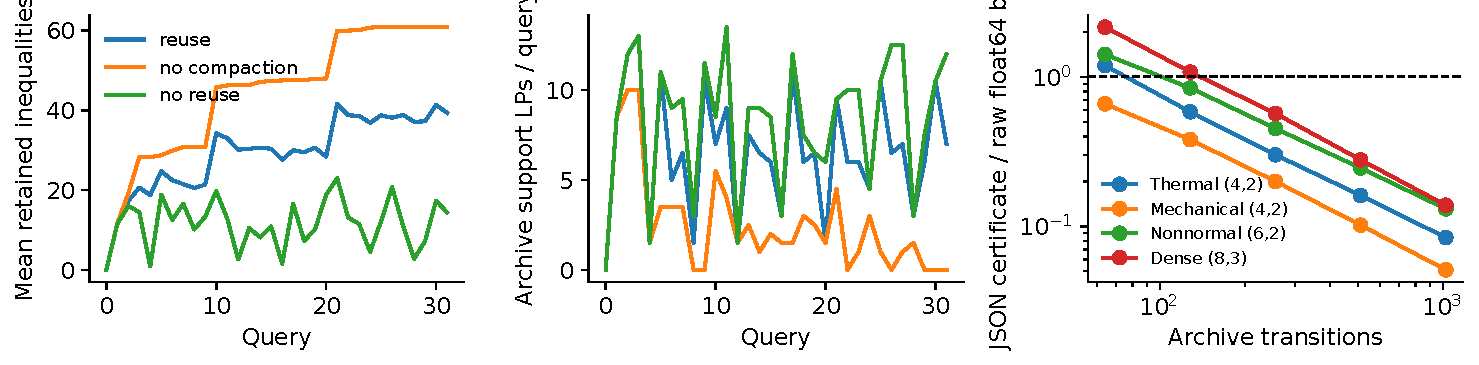
\includegraphics[width=\linewidth]{figures/ablation_streaming.pdf}
\caption{Ablations and streaming. Compaction limits retained data; reuse can reduce archive support calls relative to restarting. Payload ratios compare complete serialized controller certificates, including prior constraints and row witnesses, with raw transition arrays in float64. They are representation-size proxies, not measured network traffic or process memory.}\label{fig:ablation}
\end{figure}
\subsection{Stale-witness counterexample}
A scalar example isolates this issue without restricting the main method. Let $A=0$, $B\in[0.5,1.5]$, $\eta=0.1$, $x=0$, $v=1$, and $\bar u=0.8$. The old transition $(u,y)=(0.1,0.1)$ does not tighten the prior. The safe action is $0.6$, with cost $0.08$; the feasible old witness $B=1.5$ gives the same optimistic cost. A new transition $(u,y)=(1,0.5)$ restricts $B$ to $[0.5,0.6]$. The new full-data action is $0.8$, with cost $0.02$. Unscreened reuse would certify zero gap for a decision whose actual gap is $0.06$. The new transition can be collected in a separate identification experiment; it is not claimed to satisfy the later deployment input bound. The supplied executable example reproduces the numbers including numerical margins.

\subsection{Proof of Proposition~\ref{prop:polygon}}
\begin{proof}
For any $N\geq4$, let $z_j=(\cos(j\pi/N),\sin(j\pi/N))$, $j=0,\ldots,N-1$, $y_j=0$, $\eta=1$, and prior $[-3,3]^2$. The true row parameter is zero. Independently reset one-step experiments realize these regressors and zero disturbances. Each slab $|z_j^\top\theta|\leq1$ defines two distinct sides of a regular $2N$-gon. Removing that transition increases the support in direction $z_j$, since the adjacent facet intersections lie strictly beyond its removed side. All $N$ transitions are thus necessary for exact uniform support preservation.
\end{proof}


\paragraph{Scope of computational evidence.}
A data subset's robust support upper bound is also an upper bound for the full model. The primary audit checks these support bounds and the true model's worst bounded-noise successor at every method-query evaluation; it does not claim exhaustive enumeration of all full-matrix vertices. The full-data comparator is independently optimized at every common query. Its finite-cut dual and robust feasible action are checked by the same support-exchange solver, while small analytic tests provide an independent optimization check. Larger-scale solver equivalence is empirical, not a formal proof of software correctness.

\paragraph{Reproduction.}
The repository contains all source, the frozen plan and amendments, seed/configuration generators, raw primary histories, query/action arrays, trajectory archives, summary tables, figures, and a result audit. Run \texttt{python3 -m unittest discover -s tests -v}, then the benchmark scripts described in the README, and finally \texttt{python3 analyze.py}. Run \texttt{tectonic main.tex} in \texttt{paper/} to rebuild the manuscript. Wall times vary with hardware and concurrent workloads; scientific comparisons should exclude timing fields. A release checksum manifest identifies the exact delivered data and manuscript sources.
\end{document}
